\documentclass[../sparc.tex]{subfiles}
\graphicspath{{\subfix{../images/}}}
\begin{document}

%%%%%%%%%%%%%%%%%%%%%%%%%%%%%%%%%%%%%%%%%%%%%%%%%%%%%%%%%%%%%%%%%%%%%%%%%%%%%%%%
\newpage
\subsection{Двумерные массивы}
\index{Программирование!Массив!Двумерный массив}

Было бы круто разместить наши ноты таким образом, чтобы каждая нота лежала в
ячейке массива вместе со своей длительностью. К счастью, у нас есть такая
возможность -- мы можем использовать \emph{двумерные массивы}.

Схематическое изображение двумерного массива представлено в виде таблицы
\ref{table:array-example-2}.

\begin{table}[ht]
  \centering
  \begin{tabular}{r|l|l|l}
    \multicolumn{1}{l}{№ строки} & \multicolumn{2}{l}{№ столбца}                 &   \\
    \multicolumn{1}{l}{}         & \multicolumn{1}{l}{0} & \multicolumn{1}{l}{1} &   \\ 
    \cline{2-3}
    0                            & с4                    & 4                     &   \\ 
    \cline{2-3}
    1                            & с4                    & 4                     &   \\
    \cline{2-3}
    2                            & g4                    & 4                     &   \\
    \cline{2-3}
    3                            & g4                    & 4                     &   \\
    \cline{2-3}
    4                            & a4                    & 4                     &   \\
    \cline{2-3}
    5                            & a4                    & 4                     &   \\
    \cline{2-3}
    6                            & g4                    & 2                     &   \\
    \cline{2-3}
  \end{tabular}
  \label{table:array-example-2}
\end{table}

Каждая строка нашего массива должна содержать описание одной ноты. Столбец с
номером ноль содержит частоту ноты, а столбец номер один содержит её
длительность в виде знаменателя простой дроби, где в числителе у нас находится
длина такта. Например, нота номер ноль (``C4'') имеет в музыкальном произведении
длительность $\frac{1}{4}$, следовательно её длительность будет записана, как 4.

Записать программно мелодию в виде двумерного массива можно следующим образом:

\begin{minted}{cpp}
float melody[28][2] = {
  {c4, 4}, {c4, 4}, {g4, 4}, {g4, 4},
  {a4, 4}, {a4, 4}, {g4, 2},
  {f4, 4}, {f4, 4}, {e4, 4}, {e4, 4},
  {d4, 4}, {d4, 4}, {c4, 2},
  {g4, 4}, {g4, 4}, {f4, 4}, {f4, 4},
  {e4, 4}, {e4, 4}, {d4, 2},
  {g4, 4}, {g4, 4}, {f4, 4}, {f4, 4},
  {e4, 4}, {e4, 4}, {d4, 2},
};
\end{minted}

Как можно видеть, теперь каждый элемент массива -- это по сути одномерный массив
из двух элементов, записанный в фигурных скобках. Например, элемент номер ноль
нашего массива \texttt{melody} содержит массив \texttt{\{c4, 4\}} -- частота ноты
и её длительность.

Теперь мы можем адаптировать код воспроизведения мелодии под наши задачи:

\begin{minted}{cpp}
// ...

void loop() {
  const long BPM = 120;
  const long MINUTE = 60 * 1000000;
  const long T = (MINUTE / BPM) * 4;

  for (int note_idx = 0; note_idx < 28; note_idx++) {
    play_tone(SPEAKER_PIN,
              melody[note_idx][0],
              T / melody[note_idx][1]);
    delay(100);
  }
}
\end{minted}

Используя двумерные массивы, можно кратко и ёмко описать мелодию, даже намного
более сложную, чем ``Twinkle, Twinkle, Little Star''.

На этом этапе нам необходимо разобрать, как же работает \emph{нотный стан}
(называемый также \emph{нотоносцем}), на котором располагаются ноты -- для того,
чтобы уметь самостоятельно определять, где какая нота (частота) находится.

\section{Нотный стан}
\index{Музыка!Нотный стан (нотоносец)}

Мы можем программировать простые мелодии, не зная нотной записи (например,
используя готовые примеры из интернета) и для большинства популярных мелодий
(вроде ``Имперского марша'' из ``Звёздных войн'') найти ноты в научной нотации
(или даже готовые программы для Arduino!) не составит труда. Но в какой-то
момент мы можем столкнуться с ситуацией, когда для нашей любимой мелодии есть
только ноты и более ничего.  Поэтому, прежде чем двигаться дальше, неплохо бы
остановиться на нотной записи.

Посмотрим ещё раз на мелодию ``Twinkle, Twinkle, Little Star''.

\begin{figure}[ht]
  \centering
  \begin{lilypond}
    \relative c' {
      \numericTimeSignature
      \time 4/4
      c4 c g' g
      a a g2
      f4 f e e
      d d c2
      g'4 g f f
      e e d2
      g4 g f f
      e e d2
      c4 c g' g
      a a g2
      f4 f e e
      d d c2
    }
    \layout {
      indent = 0\mm
      line-width = 100\mm
      ragged-last = ##t
    }
  \end{lilypond}
  \label{fig:sound-fig-4}
  \caption{``Twinkle, Twinkle, Little Star''}
\end{figure}

Ранее мы проигнорировали расположение нот по оси ``Y'' и вместо этого
использовали готовые буквенные обозначения. Теперь пришло время внимательно
посмотреть на эти группы по пять линий и обозначения на них.

Начнём с линий -- они называются \emph{нотным станом} (его также называют
``нотоносцем'', поскольку он ``несёт'' на себе ноты.)

\index{Музыка!Скрипичный ключ}
Поверх нотного стана записываются ноты и другие обозначения. В самом начале
линий пишется большая закорючка, называемая \emph{ключом} -- ключ определяет
положение определённой ноты на нотном стане. Выше в мелодии ``Twinkle, Twinkle,
Little Star'' используется только один из видов ключа -- называемого
\emph{скрипичным ключом}. Скрипичный ключ обводит кружочком-завитком ту линию,
на которой располагается нота ``соль'' четвёртой октавы (``G4''):

\begin{figure}[ht]
  \centering
  \begin{lilypond}
    \relative c' {
      \numericTimeSignature
      \time 4/4
      g'1
    }
  \end{lilypond}
  \label{fig:lilypond-clef-example}
  \caption{Скрипичный ключ и нота ``G4''.}
\end{figure}

Как можно видеть на рисунке выше, вторая линия снизу соответствует ноте ``Соль''
-- поскольку она обведена скрипичным ключом. Следовательно, все ноты, которые
``зацепились'' за эту линию, будут нотой ``Соль'' четвёртой октавы (``G4''.)

Но ноты могут записываться не только на самих линиях, но и посерёдке между ними.

Схематически расположение нот можно представить в виде графика, как на
рис. \ref{fig:lilypond-music-graph-1}.

\begin{figure}[ht]
  \centering
  \begin{tikzpicture}
    \node (image) at (2, 0) { \resizebox{1.0\textwidth}{!}{
        \begin{lilypond}
          \relative c' {
            \numericTimeSignature
            \time 4/4
            c8 d8 e8 f8 g8 a8 b4
          }
        \end{lilypond}
      }
    };
    \foreach \n [count=\i, evaluate=\i as \y using real(\i / 2.6)] in {
      C4, E4, G4, B4, D5, F5
    } {
      \node at (-3.3, \y - 1.6) {\tiny \n};
    };
    \foreach \n [count=\i, evaluate=\i as \y using real(\i / 2.6)] in {
      D4, F4, A4, C5, E5, G5
    } {
      \node at (-3.0, \y - 1.4) {\tiny \n};
    };
    \draw[thick, ->] (-4.0, -2.0) -- (8.0, -2.0) node[anchor=north east] {x};
    \draw[thick, ->] (-4.0, -2.0) -- (-4.0, 1.5) node[anchor=north east] {y};
  \end{tikzpicture}
  \label{fig:lilypond-music-graph-1}
  \caption{Музыкальный ``график''.  По оси ``x'' отложено время, по оси ``y'' --
    частота звука.}
\end{figure}

На данном ``музыкальном'' графике по порядку выстроены ноты ``C'', ``D'', ``E'',
``F'', ``G'', ``A'', ``B''. При движении вверх по оси ``y'', частота звуков
повышается, при движении вниз -- понижается.

Следовательно, если мы будем двигаться выше по линейкам, то между второй снизу и
третьей линейкой (она является средней на рисунке) будет находиться следующая
нота после ``Соль'' (``G4'') -- а именно нота ``Ля'' (``A4''). Третья же линейка
(средняя) соответствует ноте ``Си'' (``B4'') и так далее. Если мы пойдём ещё
выше, от над средней линейкой находится уже начало следующей, пятой октавы -- то
есть, нота ``До'' (``C5''.)

Если будем двигаться вниз от ноты ``Соль'' четвёртой октавы, то будем идти в
обратную сторону: между первой снизу и второй линией находится нота ``Фа''
(``F4''), самая первая (нижняя) линия соответствует ноте ``Ми'' (``E4''.)

Для того, чтобы запомнить расположение нот на нотном стане, можно
воспользоваться ``запоминалками'' -- мнемониками. В интернете их можно найти
великое множество.  Наш вариант мнемоники для скрипичного ключа показан на рис.
\ref{fig:lilypond-music-clef-mnemonic}.

\begin{figure}[ht]
  \begin{tikzpicture}
    \node (image) at (4, 2) {
      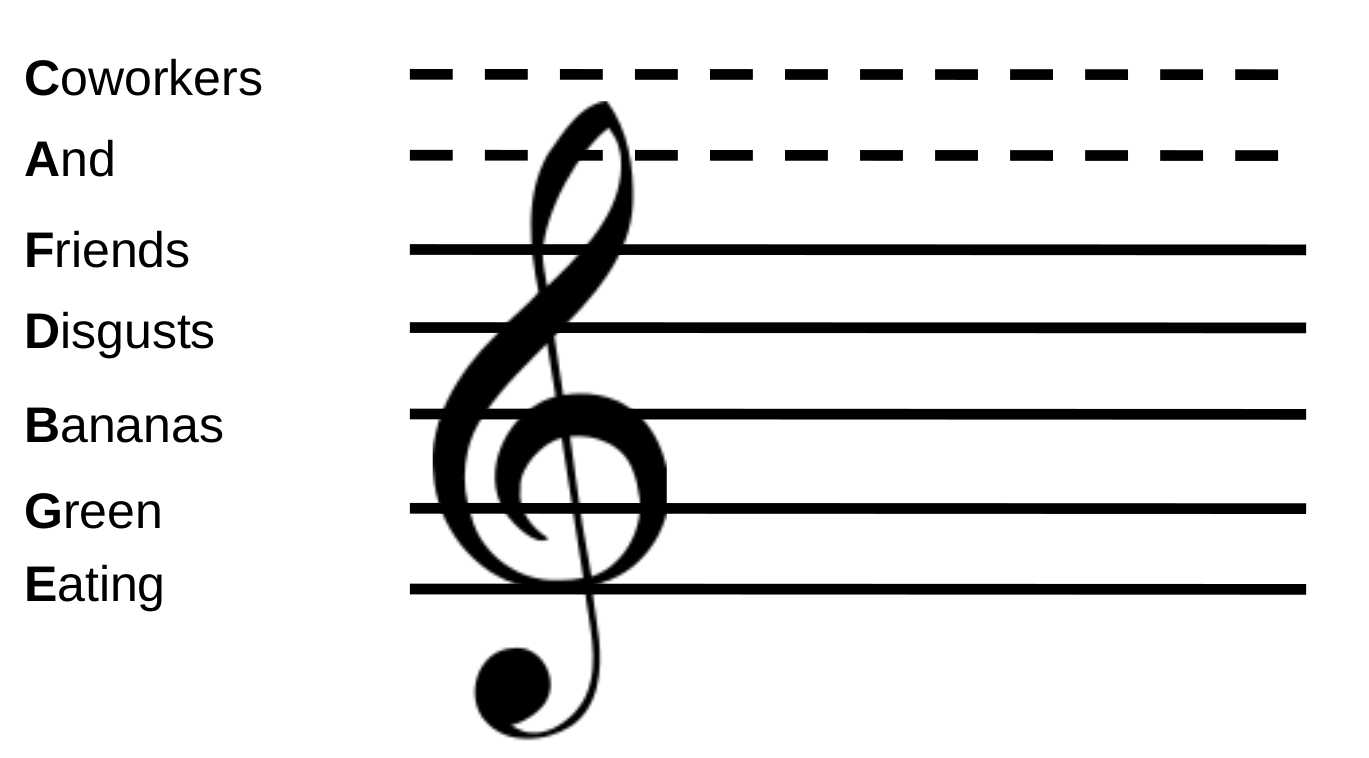
\includegraphics[width=8cm]{music-clef-mnemonic}
    };
    \draw[thick, ->] (0, -1.0) -- (10, -1.0) node[anchor=north east] {x (Время)};
    \draw[thick, ->] (0, -1.0) -- (0, 4.0) node[anchor=north east] {y (Частота)};
  \end{tikzpicture}
  \label{fig:lilypond-music-clef-mnemonic}
  \caption{Мнемоника для запоминания расположения нот в скрипичном ключе.}
\end{figure}

Если читать слова снизу вверх, то образуется фраза ``\textbf{E}ating
\textbf{G}reen \textbf{B}ananas \textbf{D}isgusts \textbf{F}riends \textbf{A}nd
\textbf{C}oworkers'' (``Поедание зелёных бананов вызывает отвращение у друзей и
коллег по работе''). Первая буква слова кодирует ноту в научной нотации. Вверху
мы, помимо основных пяти линеек, подрисовали ещё две дополнительных линии,
выделив их пунктиром. На нотном стане дополнительные линии сверху и снизу
добавляются, если не хватает основных линий для записи композиции. Мнемоника
кодирует только основные линии нотного стана, однако зная их, мы можем понять,
какие ноты находятся между линиями.

\end{document}
